\FloatBarrier
\subsection{Recursive Neural Tensor Networks}
% pros and cons of each method considered
There are many possible forms for a neural network that classifies jets;
\begin{itemize}
    \item A feed forward Deep Neural Network (DNN). This is simple to train but requires a fixed length input.
        Obtaining a fixed length input is a challenge because the number of tracks in a jet is not fixed,
        expert features must be used, and often some form of interpolation or padding is required. 
        This doesn't make a DNN a very natural fit for the problem.
    \item A Convolutional Neural Network (CNN). This can be run on an image generated by the calorimeter output.
        It has the advantage of interpretability because the filters it developed to scan the image can be analysed and some of it's process can be estimated.
        Removing symmetries from the images, however, is difficult to achieve without distorting their physical content.
        Rotations in particular are frequently done improperly, altering the jet mass.
        Further, the images are sparse, and a CNN focuses on local correlations so cannot perform optimally on spares images.
    \item A Recurrent Neural Network (RNN). This can read in a sequence, so if we could order the tracks it would be able to used all there data.
        Finding a natural ordering for the tracks is difficult, however.
        Previously \(p_T\) has been used, the Lund Plane is certainly a natural ordering,
        but it doesn't capture all the tracks.
    \item A Recurrent Neural Tensor Network (RTRN). RTRNs follow a tree shape, being originally developed for parsing syntax trees.
        This happens to coincide exactly with the shape of a jet clustering algorithm, so we could apply them to this.
\end{itemize}
% add something about all the thoughts on zero padding
To begin with the starting point considered was DeepCSV. It is a DNN, so it's foible is a fixed length input vector.
As each input is one jet long, two types of variable are considered, variables that describe an aspect of the jet as a whole
(\(p_T\) of the jet for instance) or variables that describe an aspect of a single track (such as \(p_T\) of that track).
The first kind have a fixed length and provided all values are successfully reconstructed (which is not always true)
will require no `padding'.
Padding is the manner in which missing values are filled.
The second kind, variables per track, will not have a fixed length even if the reconstruction is perfect because the number of tracks in a jet varies.
Unless the plan is to train a separate DNN for each size of jet (which would be statistically wasteful and computationally expensive)
some form of padding will have to be chosen.

The amount of padding required for a restricted set of tracks in my dataset is shown in figure~\ref{fig:prog_unreconstructed}.
\begin{figure}
    \centering
    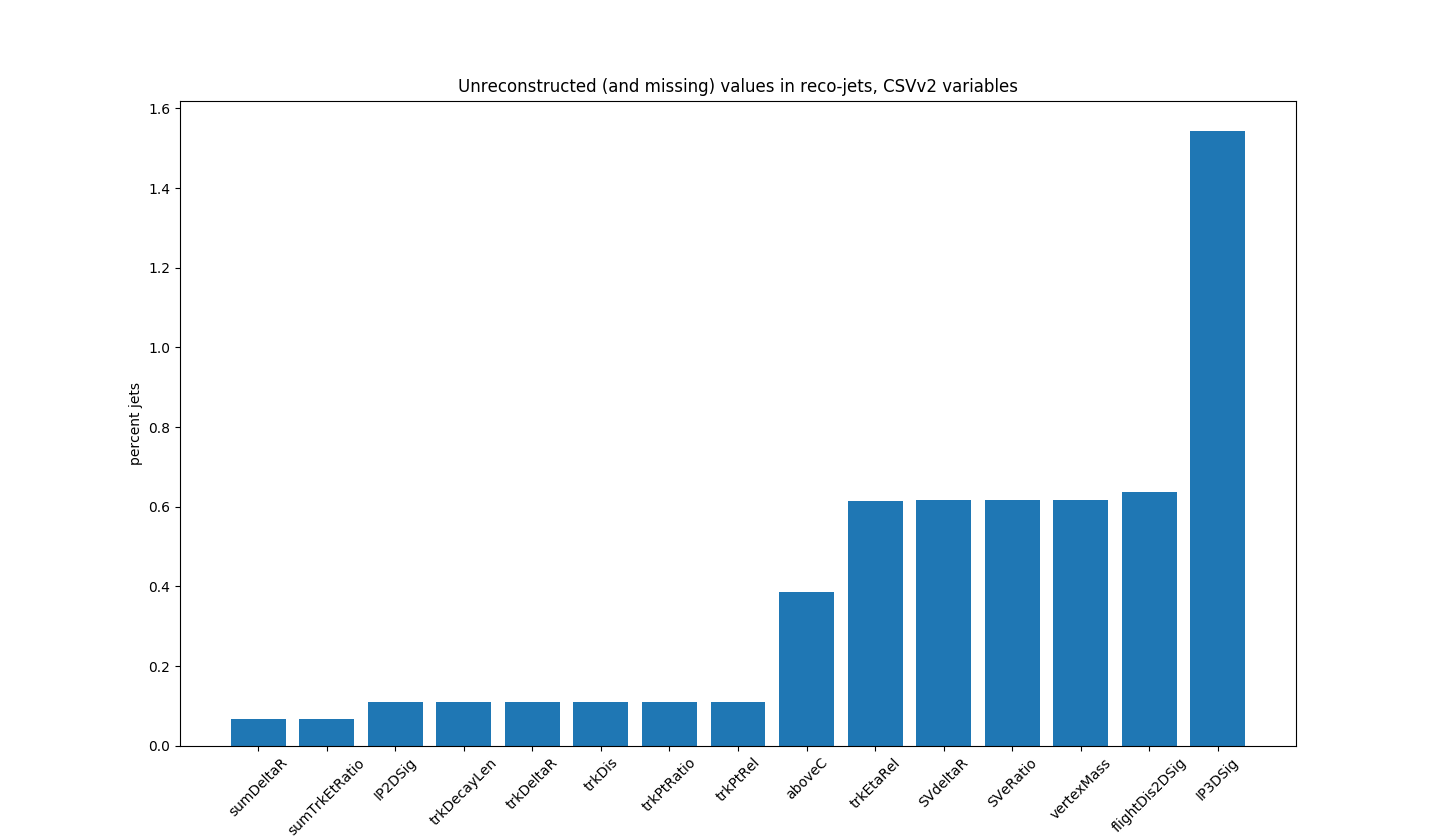
\includegraphics[width=0.8\textwidth]{images/prog_unreconstructed.png}
    \caption{Both DeepCSV and CSVv2 used zero padding to fill in values that were not available from the data. In my data sample the percentage of each variable that must be zero padded for CSVv2 is shown here.}
    \label{fig:prog_unreconstructed}
\end{figure}

The padding decision taken in~\cite{CMS_CSVDeepCSV13TeV} was called zero padding, 
but as the distributions are all centred on zero before padding this is equivalent to padding with the average value of each distribution.
Thus we can imagine that we are inserting ``average" tracks into each event until there are sufficient tracks to fill the fixed length input.
This make very little physical sense; the momentum of the additional tracks will contradict the momentum of the jet, and the angle of the tracks
will have no relation to the angle of the jet at all.

This was deemed to be an undesirable approach, so new methods that didn't require fixed length input were considered.

\subsubsection{Picture from the Monte Carlo}

In order to better envision a good neural network some time was spend graphing the behaviour of a selection of Monte Carlo showers and their jets.
A shower from a heavy Higgs decay can be seen in figure~\ref{fig:prog_bjetShower}.
Here showers are considered to start with the particles that leave the hard event, and any child of the proton beam besides the hard interaction.
These are dubbed originating particles. 
Any descendant of an originating particle is in the originating particle's shower.
Due to the requirements of colour confinement, if any originating particle is colour charged it must share descendants with another shower
so that the final descendants are colour neutral.
This happens in hadronisation.

\begin{sidewaysfigure}
    \centering
    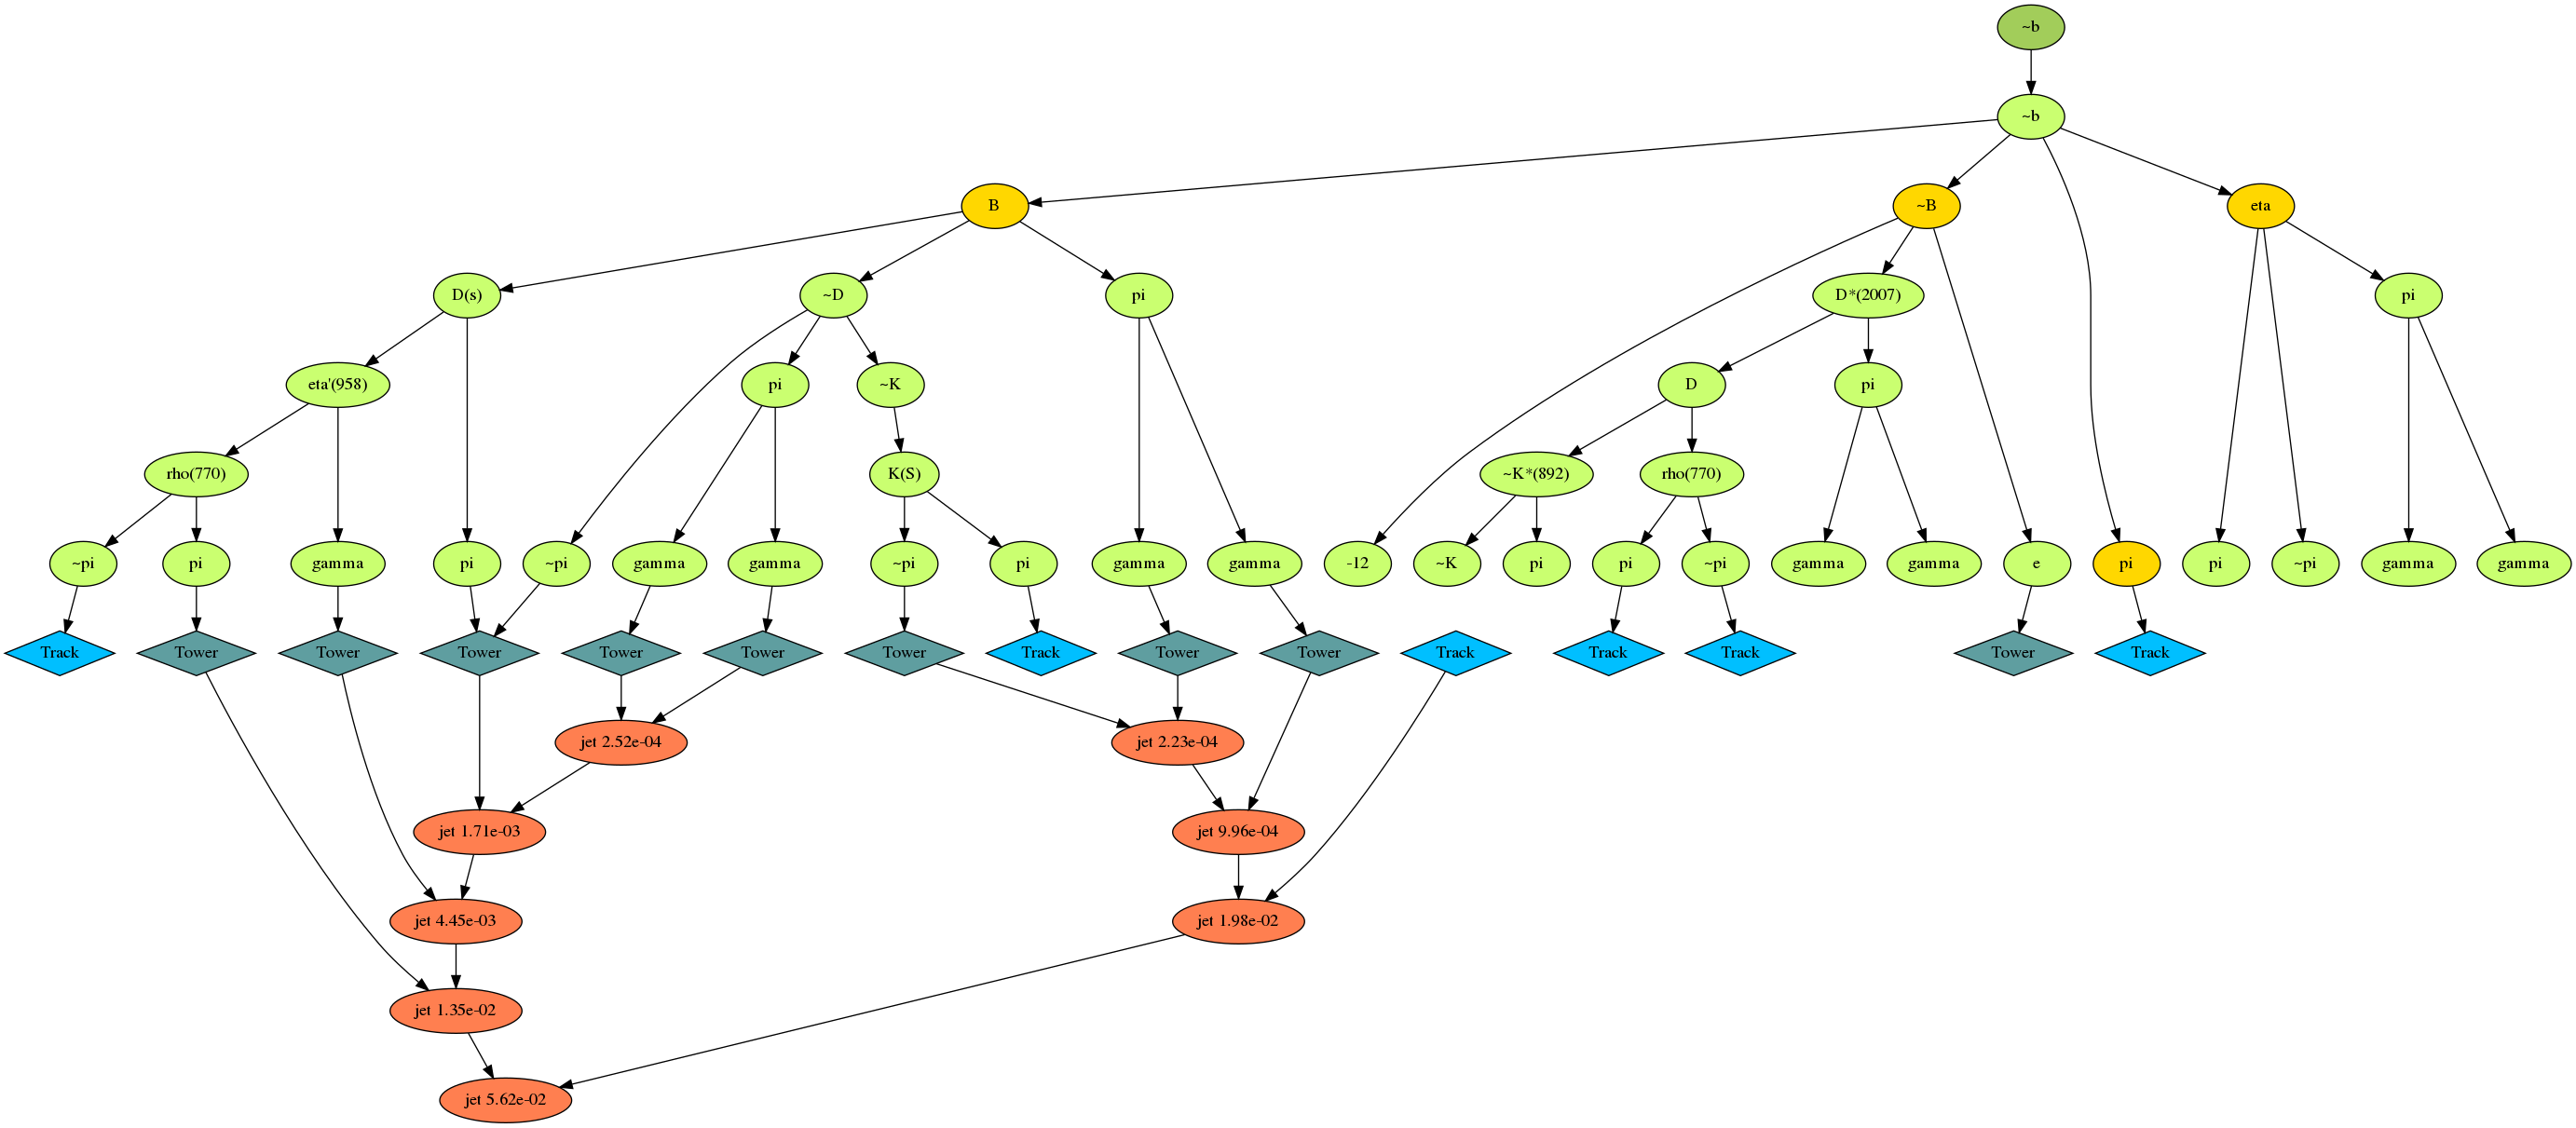
\includegraphics[width=1.\textwidth]{images/prog_bjetShower.png}
    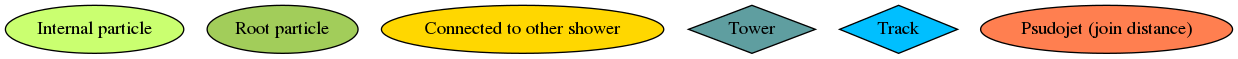
\includegraphics[width=0.5\textwidth]{images/prog_legend.png}
    \caption{A jet attempts to capture the observables let by one shower. Here we see an example shower generated in Monte Carlo.
        It was generated with aid of Madgraph~\cite{alwall_madgraph2011}, Pythia~\cite{sjostrand_pythia2015} and Delphes~\cite{deFavereau_delphesA2014}.
             The shower, and it's Monte Carlo truth is shown at the top, at the bottom
             the process of the jet clustering algorithm is seen.
         The jet clustering algorithm captures most but not all of the shower, and it captures some tracks from other parts of the event.}
    \label{fig:prog_bjetShower}
\end{sidewaysfigure}


There were a few casual observations made at this point. 
In most events, the graph of all showers is fully connected,
that is to say that the hadronisation links all showers to all other showers in most cases.
Information in one part of an event might be expected to be strongly dependant on information in the rest of the event.
This favours dealing with the event as a whole instead of jet by jet.

\begin{figure}
    \centering
    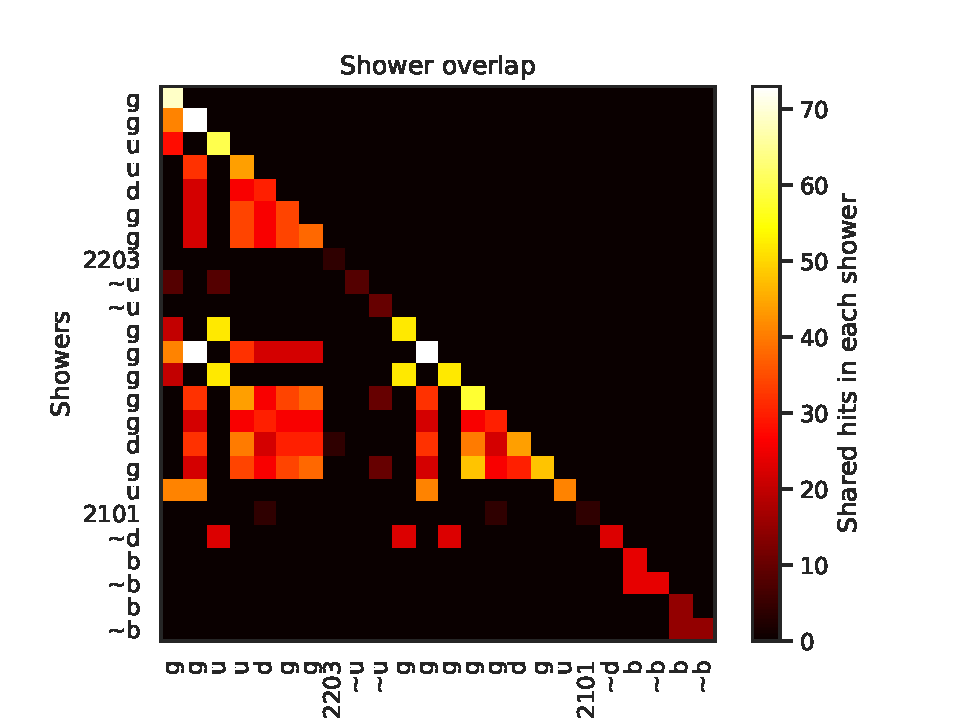
\includegraphics[width=0.8\textwidth]{images/prog_showerOverlap.pdf}
    \caption{The overlap between showers in one event. A shower is defined here as all the descendants of a particle who's parents are of the hard interaction or the proton beams.
            The axis labels identify the originating particle of the shower.
         Particles in one shower will interact with particles in another shower and then produce common descendants.
         For a shower from a colour charged this is required to form 
     colour neutral end products.}
    \label{fig:prog_showerOverlap}
\end{figure}

It also indicates that a non exclusive jet formula might make more sense - if tracks can belong to multiple showers, perhaps they should be able to belong to multiple jets.
This overlap between showers is shown for one event in figure~\ref{fig:prog_showerOverlap}.
One promising feature of this plot is that shared descendants between soft gluon showers and hard b quark showers is minimal,
so exclusive jets will merge b showers, but it looks possible to avoid excessive merging of b quark showers and soft showers.

\begin{figure}
    \centering
    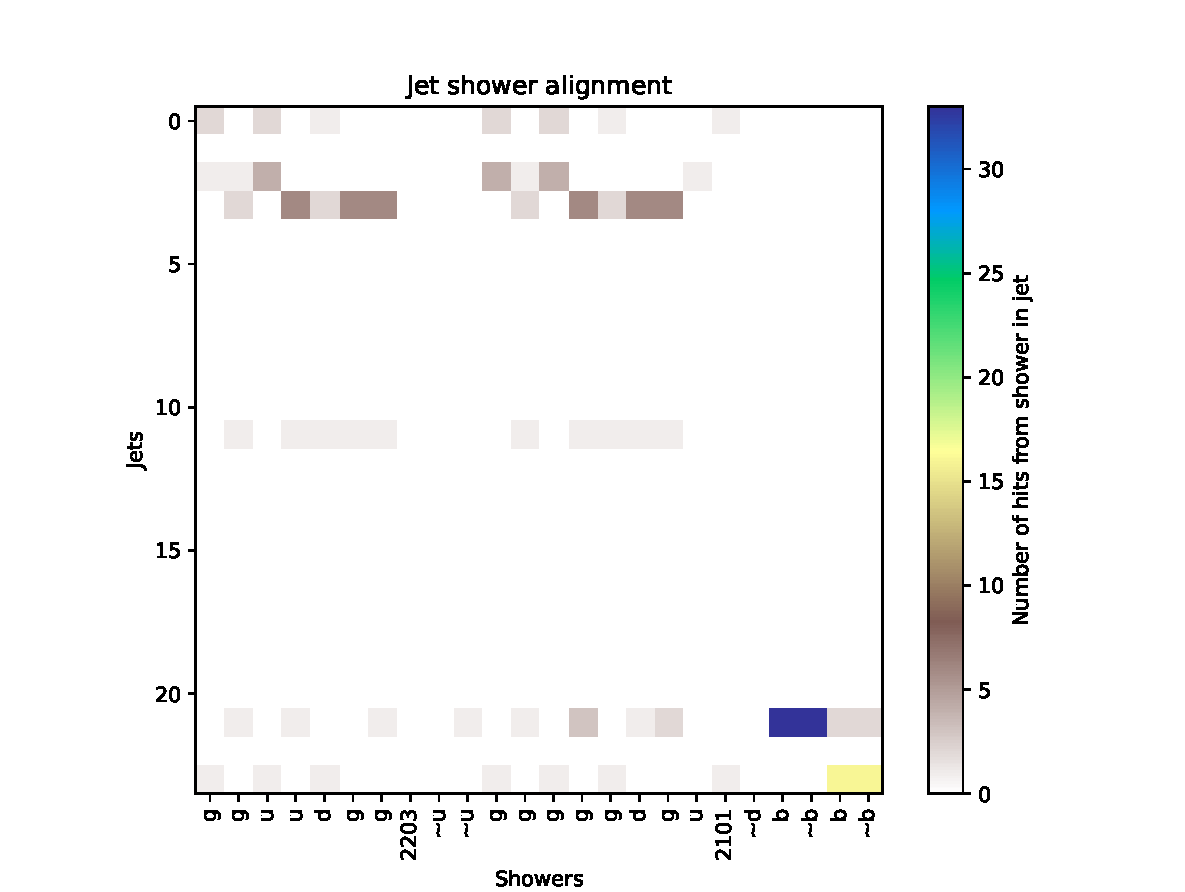
\includegraphics[width=0.8\textwidth]{images/prog_showerJetAlignment.pdf}
    \caption{The alignment between showers and jets for one event.
        The shower axis identifies the originating particle of the shower,
        the jets themselves are ordered to make the plot as close to diagonal as possible.
        Ideally each jet would capture exactly one shower
    if this occurred the plot would be diagonal.
             What is seen in this event is that many shower have be incorrectly split between many jets.}
    \label{fig:prog_showerJetAlignment}
\end{figure}

Another picture of the distinction between the signal and the soft jets can be seen in figure~\ref{fig:prog_showerJetAlignment}.
It can be seen that the hard showers fall into two jets in the bottom right of the heatmap,
and the soft showers are spread over many jets. 
This is strikingly different behaviour and one might imagine that the structure of the jet is sensitive to the nature of the shower it is built on.

It can be seen in figure~\ref{fig:prog_bjetShower} that the jet structure is not a mirror of the shower.
So the relationship between jet structure and physics is not immediately obvious, but perhaps it would be a useful structure for a classifier to combine information.
This is the inspiration for the plan to use RNTNs.


\subsection{Architectural direction}
The network used by~\cite{cheng_recursive_2018} was originally developed for parsing syntax trees.
It the case of jet clustering it generates a state vector (\(\vec{h}_k\)) for every pseudojet.
That state vector encodes the useful information about the pseudojet structure and kinematics.

The equations involved can be seen in figure~\ref{fig:plan_treeTagger}.
Qualitatively the first pseudojets being the tracks or towers must make a state vector out of the observables alone.
These are known as leaf nodes in the net, and they learn a process for encoding observables into a new hidden state.
When two pseudojets merge into a new pseudojet there are three kinds of input to the state vector;
the left and right state vectors of the child nodes and the combined kinematics of the pseudojet.
A separate procedure is learnt to combine these three things.
These two processes combine all the tracks into one root state vector.

The root state vector, or final state vector, will be passed on to a DNN,
along with global event information which tags the jet.


\begin{figure}
    \centering
    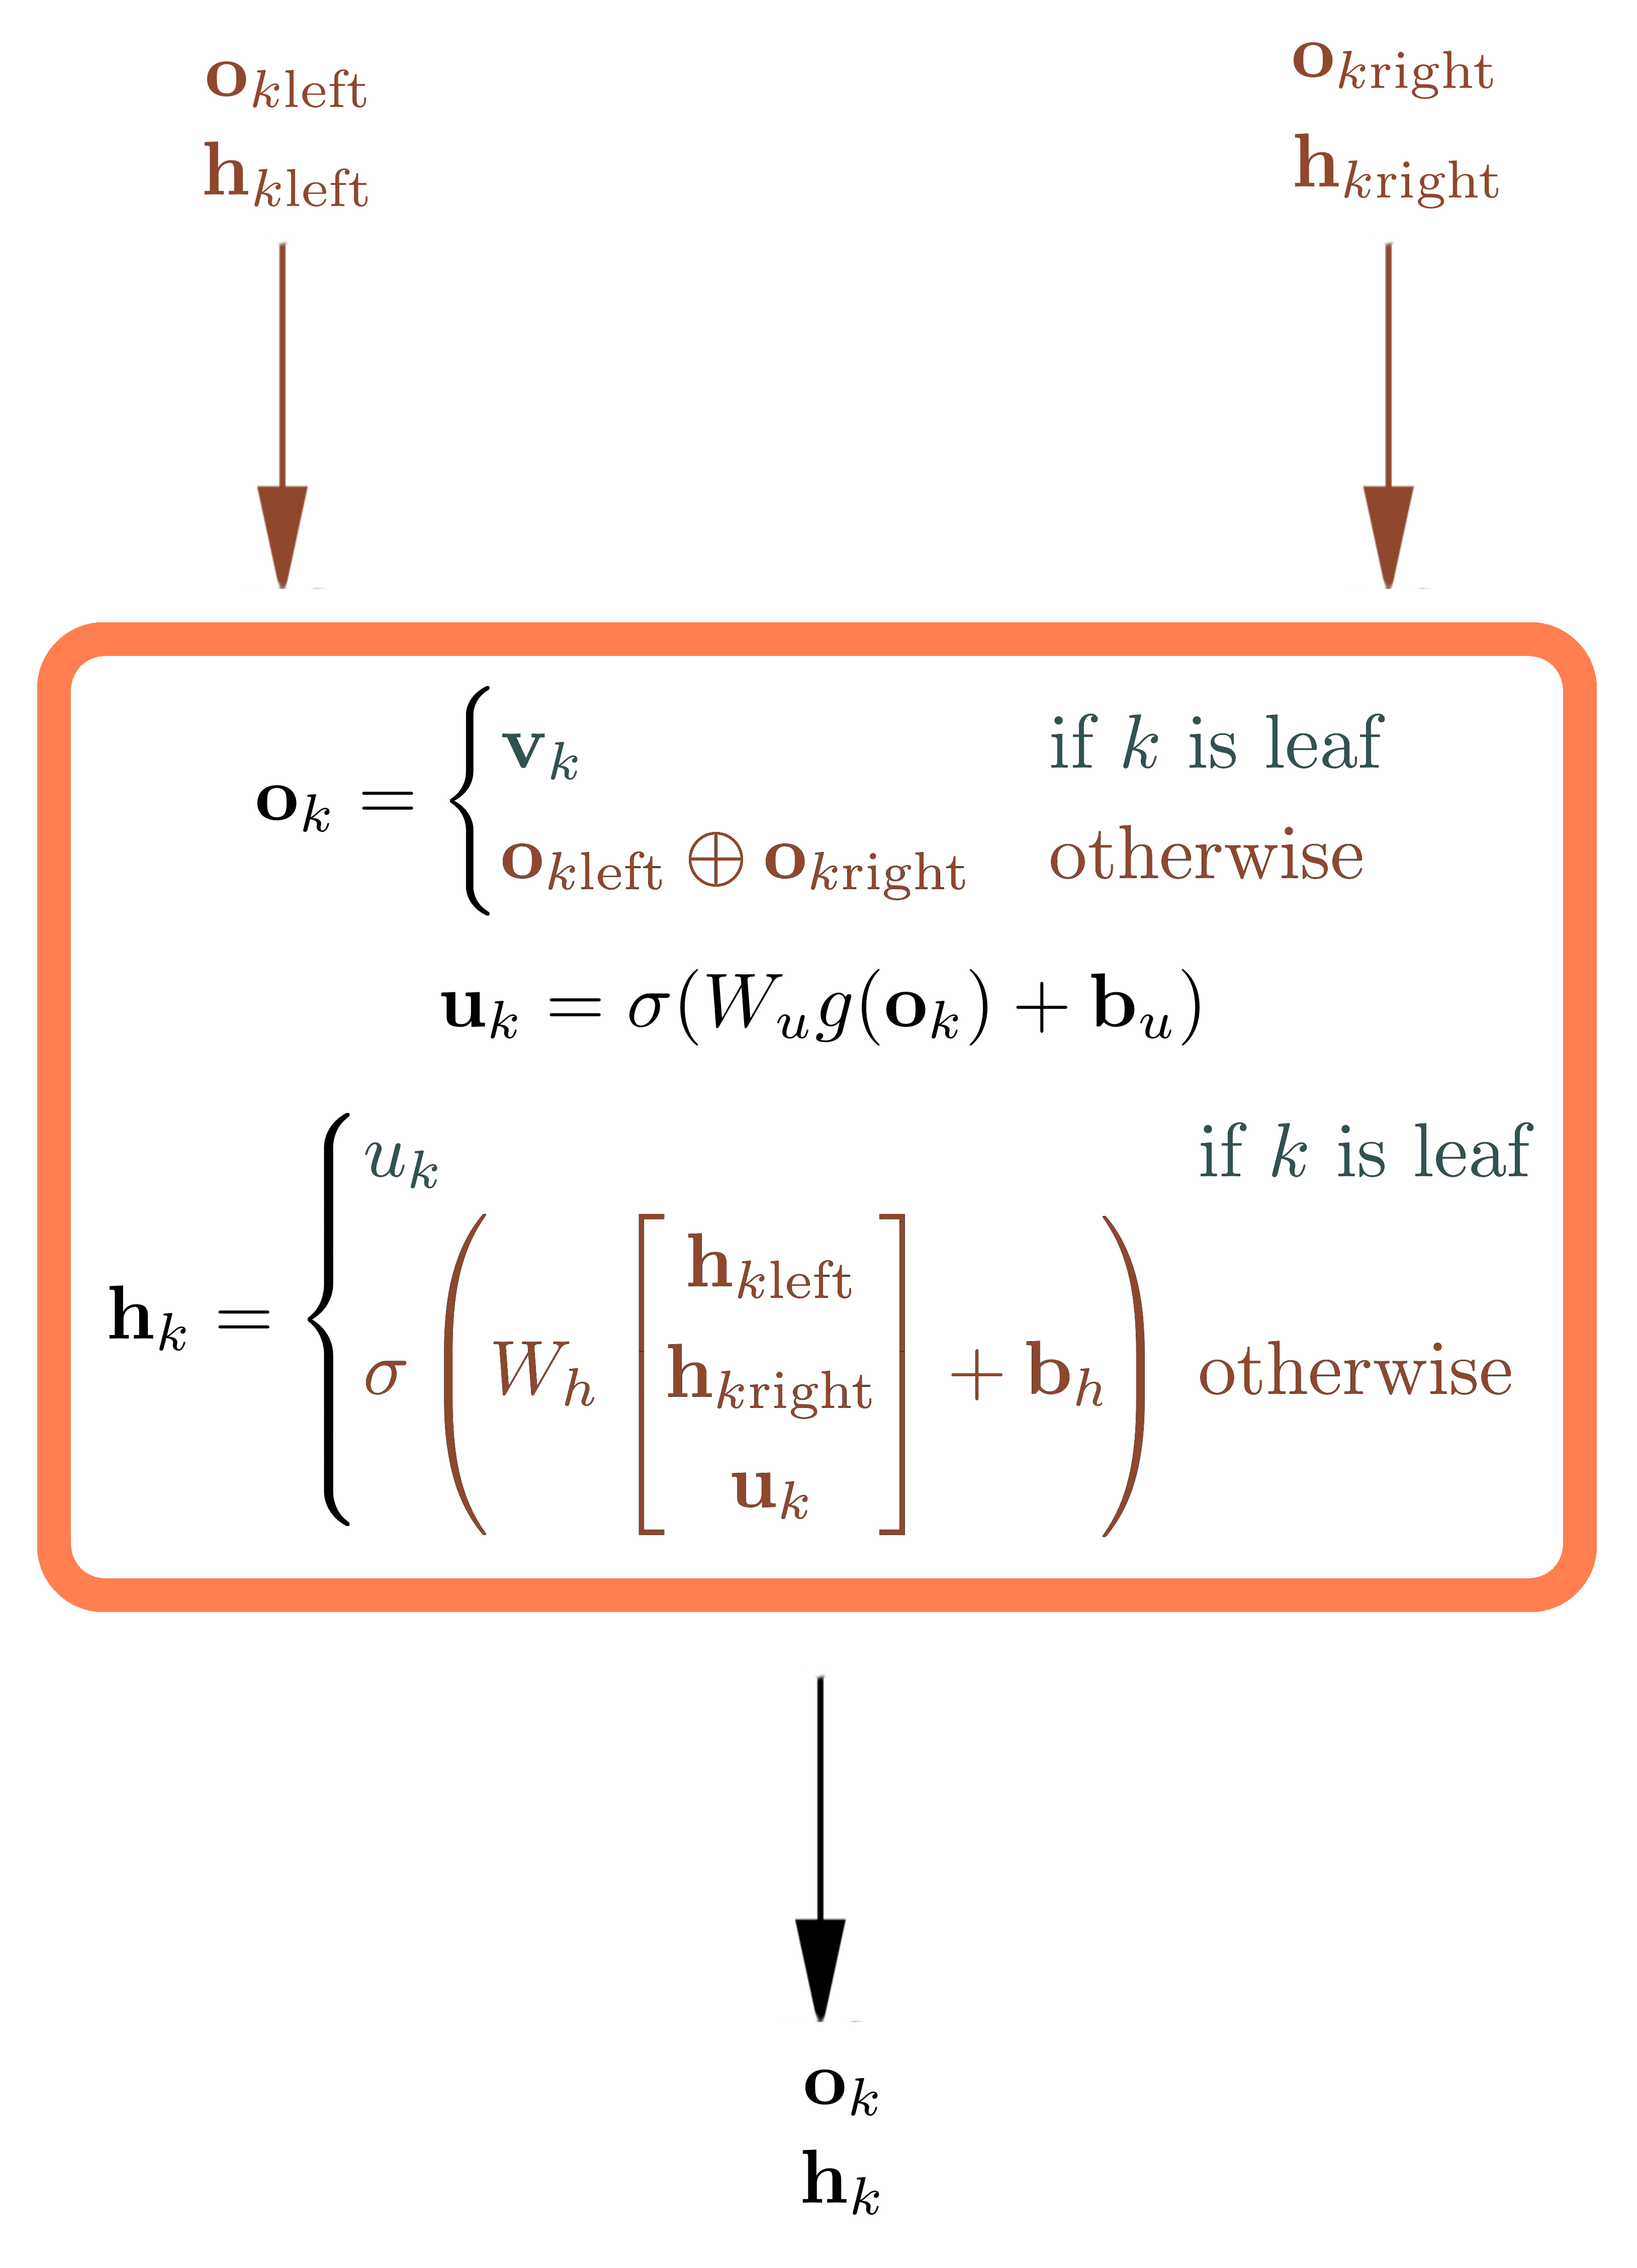
\includegraphics[width=0.5\textwidth]{images/plan_treetagger.png}
    \caption{A single node of an RNTN.
        The vector \(\vec{o}_k\) is the vector of observable properties of the \(k^\text{th}\) node. 
        If the \(k^\text{th}\) node is a leaf then these would be the track properties, otherwise they are a combination of the properties of the tracks below \(k\).
        The vector \(\vec{u}_k\) is the embedding of \(\vec{o}_k\) into the latent space of the net.
        The vector \(\vec{k}_k\) is the `state' of the \(k^\text{th}\) node, structural information about the tree propagates in the state of the nodes.
    }
    \label{fig:plan_treeTagger}
\end{figure}

\subsubsection{Subsequent steps}
Once this net has been replicated and seen to perform acceptably there are a number of forward direction open;
\begin{enumerate}
    \item Most RNNs and RNTNs have a target available at every node.
          This greatly improves the stability of the training process.
          A physically inspired intermediate target might be identified of increase the stability of the net as it trains.
    \item RNTNs have been implemented with Long Short Term Memory (LSTM) and jet taggers with LSTM have been implemented~\cite{Egan:2017ojy}.
      To my knowledge, however, they have yet to be combined.
      This would be a very natural extension.
    \item Such a net will be sensitive to the subtleties of hadronisation, 
        there would be a number of possibility's for testing their robsutness to Monte Calro errors.
        Unsupervised training on known signal/background regions in data could be compared to equivalent MC trained nets.
        Different MC generators could be compared.
    \item It would be interesting to find an interpretation of the net's latent space.
          Perhaps t-SNE would be suitable for this.
\end{enumerate}

Points 1 and 2 should certainly be undertaken, if the structure show promise then points 3 and 4 would be worth attempting.

